\chapter{Classification}

\section{Marge d'un hyperplan}

On considère des données labellisées linéairement séparables $(x_i,y_i)$, $y_i \in \{1,-1\}$, et un hyperplan séparateur $H$ d'équation $a^\top x + b = 0$, où $a \in \RR^n$ et $b \in \RR$. On supposera que $x_1$ et $x_2$ sont des vecteurs de support pour chacune des classes, c'est-à-dire tels que 
\eq{
	a^\top x_1 + b = 1 \qetq a^\top x_2 + b = -1.
}

\begin{enumerate}
	\item Montrer que $a$ est un vecteur normal à $H$, i.e. pour tout $x,y \in H$, $a^\top (x-y) = 0$.
	\item Montrer que pour tout point $x \in \RR^n$,
	\eq{
		d(x,H) = \frac{\abs{a^\top x + b}}{\norm{a}}
	}
	\item En déduire l'expression de la marge de $H$ en fonction de $a$.
\end{enumerate}

\paragraph{\textcolor{blue}{Solution.}}
\begin{enumerate}
	\item On a $a^\top(x-y) = a^\top x + b - (a^\top y +b) = 0 + 0 = 0$ car $x$ et $y$ appartiennent à l'hyperplan.
	\item Pour tout point $p$ de l'hyperplan $H$, on a
	\eq{
		d(x,H) = \frac{\abs{a^\top (x-p)}}{\norm{a}} = \frac{\abs{a^\top x + b - (a^\top p + b)}}{\norm{a}} = \frac{\abs{a^\top x + b}}{\norm{a}}
	}
	
	\item La marge est donnée par $d(x_1,H) + d(x_2,H) = \frac{1}{\norm{a}} + \frac{1}{\norm{a}} = \frac{2}{\norm{a}}$.
\end{enumerate}


\section{Astuce du noyau}

On considère un jeu de $8$ données labellisées $(\mathbf{x}^{(i)},y^{(i)})$, avec $\mathbf{x}^{(i)} \in \RR^2$ et $y^{(i)} \in \{-1,+1\}$, pour $i=1,\ldots,8$. Ces données sont représentées en Figure~\ref{fig:donnees}. On cherche à classsifier automatiquement ces données à l'aide de la méthode des machines à vecteurs de support (SVM).
\begin{enumerate}
	\item On rappelle qu'une SVM classique consiste à résoudre le problème d'optimisation
	\eql{\label{eq:svm}
		\min_{\mathbf{a} \in \RR^2, \; b\in \RR} \quad \frac{1}{2}\norm{\mathbf{a}}^2 \qscq y^{(i)}(\mathbf{a}^\top \mathbf{x}^{(i)} + b) \geq 1 \quad i=1,\ldots,8
	}
	\begin{enumerate}
		\item Que représentent les contraintes du problème?
		\item Que représente la fonction objectif?
	\end{enumerate}
	
	\item Expliquer pourquoi résoudre le problème \eqref{eq:svm} pour les données considérées ici ne permettra pas d'identifier les deux classes.

\item Expliquer le principe de l'astuce du noyau.

\item On applique aux données une transformation $\phi:\RR^2\to\RR^2$. Le résultat est montré en Figure~\ref{fig:transformees}. Parmi les quatre transformations $\phi$ proposées ci-dessous, laquelle conduit au résultat observé?

\begin{tabular}{ll}
\\
	(a) $\displaystyle \phi(\mathbf{x}) = \begin{bmatrix} x_1 & x_1^2+x_2^2 \end{bmatrix}$
	&
	\qquad (b) $\displaystyle \phi(\mathbf{x}) = \begin{bmatrix} x_1 & x_1+2x_2 \end{bmatrix}$\\ \\
	(c) $\displaystyle \phi(\mathbf{x}) = \begin{bmatrix} x_2 & x_1^2-x_2^2 \end{bmatrix}$
	&
	\qquad (c) $\displaystyle \phi(\mathbf{x}) = \begin{bmatrix} x_2 & x_1^2 \end{bmatrix}$
	\\ \\
\end{tabular}

\noindent Indiquer sur la Figure~\ref{fig:transformees} à côté de chaque point la donnée initiale correspondante. 

\item Représenter l'hyperplan séparateur optimal sur la Figure~\ref{fig:transformees}. Donner son équation, et déterminer sa marge. Quels sont les vecteurs de support?

\item On considère une nouvelle donnée $\mathbf{x}^{(9)} = (-1,-\sqrt{2})$ et $y^{(9)} = -1$. Représenter cette nouvelle donnée sur la Figure~\ref{fig:donnees} (on donne $\sqrt{2}\simeq 1.414$). Cette donnée sera-t-elle correctement classifiée par la SVM à noyau appris sur le jeu de données initial? Justifier votre réponse.

\begin{figure}[h!]
\centering
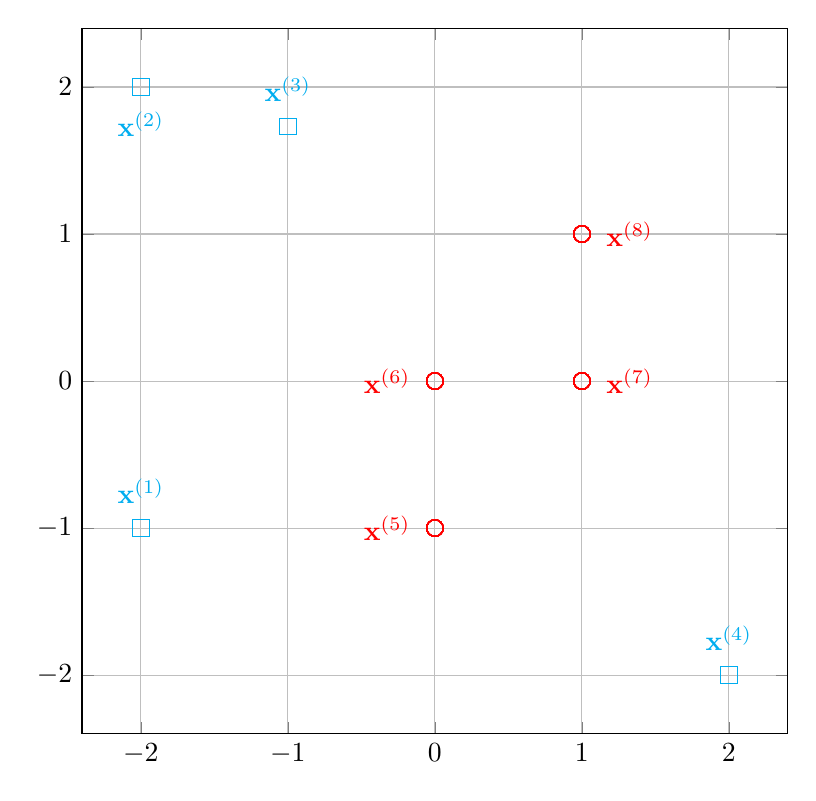
\begin{tikzpicture}
\begin{axis}[
  %cycle list={
  %  only marks,mark=o,draw=red,fill=red,mark size=3pt\\
  %  only marks,mark=o,draw=cyan,mark size=3pt\\
  %},
  %domain=0:360,
  %samples=5,
  grid,
  axis equal,
  xtick = {-2,-1,...,2},
  ytick = {-2,-1,...,3},
  width=300pt,
  height=300pt
]

%\addplot ({(1)*cos(x)},{(1)*sin(x)});
%\addplot ({(2*sqrt(2))*cos(x+45)},{(2*sqrt(2))*sin(x+45)});
\addplot[only marks,mark=square,draw=cyan,mark size=3pt]( {-2},{-1} );
\addplot[only marks,mark=square,draw=cyan,mark size=3pt]( {-2},{2} );
\addplot[only marks,mark=square,draw=cyan,mark size=3pt]( {-1},{sqrt(3)} );
\addplot[only marks,mark=square,draw=cyan,mark size=3pt]( {2},{-2} );

\addplot[only marks,mark=o,draw=red,mark size=3pt]( {1},{0} );
\addplot[only marks,mark=o,draw=red,mark size=3pt]( {0},{0} );
\addplot[only marks,mark=o,draw=red,mark size=3pt]( {1},{1} );
\addplot[only marks,mark=o,draw=red,mark size=3pt]( {0},{-1} );

\node[above] at (axis cs: -2, -0.9) {\textcolor{cyan}{$\mathbf{x}^{(1)}$}};
\node[below] at (axis cs: -2, 1.9) {\textcolor{cyan}{$\mathbf{x}^{(2)}$}};
\node[above] at (axis cs: -1, 1.832) {\textcolor{cyan}{$\mathbf{x}^{(3)}$}};
\node[above] at (axis cs: 2, -1.9) {\textcolor{cyan}{$\mathbf{x}^{(4)}$}};

\node[left] at (axis cs: -0.1, -1) {\textcolor{red}{$\mathbf{x}^{(5)}$}};
\node[left] at (axis cs: -0.1, 0) {\textcolor{red}{$\mathbf{x}^{(6)}$}};
\node[right] at (axis cs: 1.1, 0) {\textcolor{red}{$\mathbf{x}^{(7)}$}};
\node[right] at (axis cs: 1.1, 1) {\textcolor{red}{$\mathbf{x}^{(8)}$}};

%\addplot [domain=-2:2, dashed] {sqrt(4-x^2)};
%\addplot [domain=-2:2, dashed] {-sqrt(4-x^2)};

\end{axis}

\end{tikzpicture}
\caption{Jeu de données (rouge:$-1$, cyan:$+1$)}
\label{fig:donnees}
\end{figure}

\begin{figure}[h!]
\centering
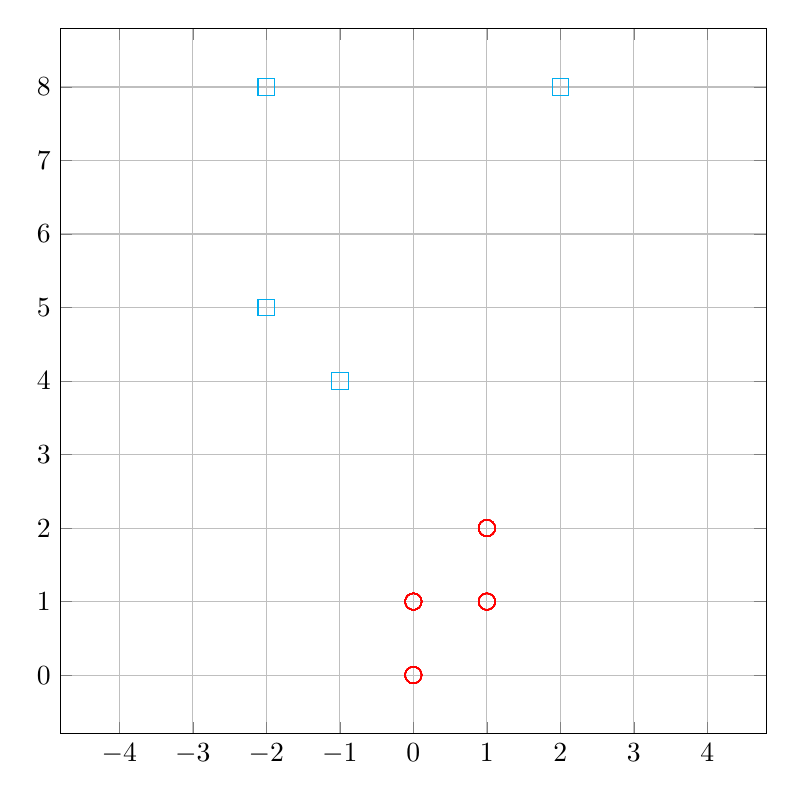
\begin{tikzpicture}
\begin{axis}[
	grid,
	ytick={0,1,...,9},
	xtick={-5,-4,...,5},
	axis equal,
	width=300pt,
	height=300pt
]
\addplot[only marks,mark=square,draw=cyan,mark size=3pt] ({-2},{5} );
\addplot[only marks,mark=square,draw=cyan,mark size=3pt] ({-2},{8} );
\addplot[only marks,mark=square,draw=cyan,mark size=3pt] ({-1},{4} );
\addplot[only marks,mark=square,draw=cyan,mark size=3pt] ({2},{8} );

\addplot[only marks,mark=o,draw=red,mark size=3pt]( {1},{1} );
\addplot[only marks,mark=o,draw=red,mark size=3pt]( {0},{0} );
\addplot[only marks,mark=o,draw=red,mark size=3pt]( {1},{2} );
\addplot[only marks,mark=o,draw=red,mark size=3pt]( {0},{1} );

\end{axis}
\end{tikzpicture}
\caption{Données après transformation}
\label{fig:transformees}
\end{figure}
	
\end{enumerate}


\section{Lagrangien}

Soit $(x_i,y_i) \in \RR^n \times \{1,-1\}$, $i=1,\ldots,p$, des données labellisées. Une SVM à marge souple consiste à résoudre le problème d'optimisation
\eq{
	\min_{\substack{a \in \RR^n \\ b \in \RR \\ \xi \in \RR^p}} \frac{1}{2}\norm{a}^2 + \alpha \sum \xi_i \qscq \xi_i \geq 0, \quad y_i(a^\top x_i + b) \geq 1 - \xi_i  \quad i=1,\ldots,p,
}
pour un $\alpha$ donné.

\begin{enumerate}
	\item Que représente les variables $\xi_i$? 
	\item Ecrire le Lagrangien $\Ll$ de ce problème.
	\item Calculer les gradients par rapport à $a$, $b$ et $\xi$ de $\Ll$. Quelle condition doivent-ils satisfaire à l'optimum?
\end{enumerate}


\paragraph{\textcolor{blue}{Solution.}}
\begin{enumerate}
	\item $\xi_i$ représente l'écart de la donnée $x_i$ du mauvais côté de la marge. Dans les SVM à marge souple, ces écarts sont autorisés mais pénalisés (par le terme $\sum \xi_i$ dans l'optimisation).
	\item Mis sous forme standard, le problème devient
\eq{
	\min \frac{1}{2}\norm{a}^2 + \alpha\sum \xi_i \qscq -\xi_i \leq 0, \quad 1 - \xi_i - y_i(a^\top x_i + b) \leq 0
}	
On a $2p$ contraintes d'inégalités: les contrainte de positivité des $\xi_i$ et les contraintes de marge. On note respectivement $\mu_i$ et $\la_i$ ($i=1,\ldots,p$) les multiplicateurs de Lagrange associés à ces contraintes. Le Lagrangien du problème est alors donné par
\eq{
	\Ll(a,b,\la,\mu) = \frac{1}{2}\norm{a}^2 + \alpha\sum \xi_i - \sum \mu_i \xi_i + \sum \la_i (1 - \xi_i - y_i(a^\top x_i + b))
}
	
	\item On a
	\eq{\begin{aligned}
			&\nabla_a \Ll(a,b,\xi,\la,\mu) = a - \sum\la_iy_ix_i\\
			&\nabla_b \Ll(a,b,\xi,\la,\mu) = -\sum \la_i y_i\\
			&\nabla_\xi \Ll(a,b,\xi,\la,\mu) = \alpha - \mu - \lambda 
		\end{aligned}
	}
	
	A l'optimum, tous ces gradients doivent être nuls. En particulier, cela implique que
	\eq{
		a = \sum \la_i y_i x_i, \quad \sum \la_i y_i = 0, \quad \mu+\la = \al
	}
	(comme $\mu$ et $\la$ doivent être positives, la dernière contraite impliquera en particulier que $0 \leq \lambda_i \leq \alpha$ pour tout $i$).
\end{enumerate}

\section{Perceptron}

On considère le réseau à deux couches représenté en Figure~\ref{fig:nn}, 
où l'on a explicitement représenté la fonction non-linéaire $\sigma$ et les biais $b_1$, $b_2$:
	\begin{figure}[h!]
	\centering
	\begin{tikzpicture}
		\node[circle,fill,inner sep=2pt,label=left:$x_1$](x1){};
		\node[circle,fill,inner sep=2pt,label=left:$x_2$,below=2cm of x1](x2){};
		\node[circle,fill,inner sep=2pt,label=left:$x_3$,below=2cm of x2](x3){};
		
		\node[circle,fill,inner sep=2pt,label=above:$z_1$,above right=1cm and 3.5cm of x2](h1){};
		\node[circle,fill,inner sep=2pt,label=below:$z_2$,below=2cm of h1](h2){};
		
		\node[above right=5mm and 2.5cm of x1,circle,fill,inner sep=2pt,label=above:$1$](b1){};
		\node[below right=5mm and 2.5cm of x3,circle,fill,inner sep=2pt,label=below:$1$](b2){};
		
		\draw[orange] (x1) -- node[above]{$w_{11}$} (h1);
		\draw[orange] (x2) -- node[above]{$w_{12}$} (h1);
		\draw[orange] (x3) -- node[above]{$w_{13}$} (h1);
		
		\draw[blue] (x1) -- node[below,near start,xshift=-2mm]{$w_{21}$} (h2);
		\draw[blue] (x2) -- node[below,near start]{$w_{22}$} (h2);
		\draw[blue] (x3) -- node[below]{$w_{23}$} (h2);
		
		\draw[dashed] (b1) -- node[above,xshift=1mm]{$b_1$} (h1);
		\draw[dashed] (b2) -- node[below,xshift=1mm]{$b_2$} (h2);
		

		\node[circle,fill,inner sep=2pt,right=2.5cm of h1] (z1) {};
		\node[circle,fill,inner sep=2pt,right=2.5cm of h2] (z2) {};
		
		\draw[dashed]  (h1) -- (z1);
		\draw[dashed]  (h2) -- (z2);
		\path[] (h1) -- node[draw,fill=white]{$\sigma$} (z1);
		\path[] (h2) -- node[draw,fill=white]{$\sigma$} (z2);
		
		\node[circle,fill,inner sep=2pt,below right= 1cm and 2.5cm of z1,label=right:$y$] (o) {};
		
		\draw[] (z1) -- node[above]{$v_{1}$} (o);
		\draw[] (z2) -- node[above]{$v_{2}$} (o);

		

		
		%\node[below right = -15pt and 5cm of h2] {$\displaystyle y = \sum_{k=1}^n v_k \, \sigma(\ww_k^\top \xx+b_k)$};
	\end{tikzpicture}
	\caption{Réseau de neurones}
	\label{fig:nn}
	\end{figure}
%

	\begin{enumerate}
	\item Exprimer les sorties intermédiaires $z_1$ et $z_2$ en fonction de l'entrée $\mathbf{x} = \begin{bmatrix} x_1 & x_2 & x_3\end{bmatrix}^\top$, des vecteurs de poids $\mathbf{w_1} = \begin{bmatrix} w_{11} & w_{12} & w_{13} \end{bmatrix}^\top$, $\mathbf{w_2} = \begin{bmatrix} w_{21} & w_{22} & w_{23} \end{bmatrix}^\top$, et des biais $b_1$, $b_2$.
	\item  Exprimer de même la sortie finale $y$ en fonction de $\mathbf{x}$ et des différents paramètres du réseau.
	\end{enumerate}

